\section{Implementation}
This section will first present the implementation of the parser for the \texttt{While} language. Then the implementations of the analysis' described in the previous section will be discussed.
\\\\
The Java language has been chosen as the implementation language.
 
\subsection{Parsing a program}
Before any analysis can take place it necessary that the program is parsed. This is done by having a parser. ANTLR is used as the framework for constructing a lexer and a parser that can take a program written in the extended \texttt{While} language and construct an abstract syntax tree (AST) using the data structures described in section~\ref{section:Abstractsyntaxtreedatastructure}. 

\subsection{Constructing the intermediate representation}
As described in section~\ref{section:CreatingFlowGraphs} we use an unbalanced tree for containing our abstract syntax tree, which serves as our intermediate representation (IR).
The implementation architecture for the IR is seen in Figure 1 - Figure 5. This architecture is mapped into java objects representing the program, each declaration, each statement etc.

\subsection{Function Mapping}
In order to access information about each statement (block) we have implemented the smallest steps of each analysis to the individual classes (blocks) in the IR.
\\\\
For each \texttt{Statement} class we have implemented following functions:
\begin{itemize}
\item Label(s) - returns the set of label for the statement 		
\item Init(s) - returns the initial label for the statement
\item Final(s) - returns the set of final labels for the statement 
\item Flow(s) - returns the flow for the statement
\item Variable(s) - returns the set of variables for the statement
\item Kill - returns the set of definitions to be killed	
\item Gen - returns the set of definitions to be generated
\end{itemize}

As an example for assignments and skip-statement we would have the following results when looking the statements \texttt{assignment} and \texttt{skip}.:
\\
\begin{tabular}{|l|l|l|}
\hline
\textbf{Statement}&		[x:=a]l&												[skip]l\\
\hline
\hline
Label(s)&		\{l\}&													\{l\}	\\
\hline
Init(s)&			\{l\}&													\{l\}\\
\hline
Final(s)&		\{l\}&													\{l\}\\
\hline
Flow(s)&		Ø&													Ø\\
\hline
Variable(s)&		variable(a)&									Ø\\
\hline
Kill&			RDentry(l)\textbackslash\{x, l' | Bl' is an assignment to A\}&		Ø\\							
\hline
Gen&				\{x, l\}&												Ø\\
\hline
\end{tabular}

We have discusses most of the function above in the previous sections of the report. However the Variable function is new. The variable function is used to get variables for a particular statement. It returns a set of variables if any is represented.

If the statement is a declaration, we have defined the variable-function as following:\\

\begin{tabular}{|l|l|}
\hline
variable(decl)&:\\
\hline\hline
(Integer)&			x -> \{x\}\\
\hline
(Array)&				A[n] -> \{A\}\\
\hline
\end{tabular}

For expressions it is defined as:
variable(expr):
	(constant) 			n -> Ø
	(variable)			x -> {x}
	(Array expr.)		A[x] -> {A} U var(x)
	(Arithmetic opr.)	a1 opa a2 -> var(a1) U var(a2)
	(Negation)			-a -> var(a)
	(Parenthesis)		(a) -> var(a)

And finally the statements:
variable(stmt):
	(Assignment) 		x := a -> {x} U variable(x)	
	(Skip)				skip -> Ø
	(Array assignment)	A[a1] := a2 -> {A} U variable(a1) U variable(a2)
	(Read)				read x -> {x}
	(Read array)		read A[a] -> {A} U variable(a)
	(Write)				write a -> variable(a)
	(composition)		S1 S2 -> variable(S1) U variable(S2)
	(if-stmt)			if b then s1 else s2 fi -> Ø
	(while loop)		while b do S od -> Ø
	
The variable-function is used for the Program Slicing algorithm.
	
The functions explained above will give us the equations that is going to be solved.

\subsection{Implementation of the analysis}
On top of the functions explained above we have implemented the algorithms which is able to perform the analysis as Reaching definitions, Program slicing, detection of signs and interval analysis. 
Mode details of each analysis is explained below.

Implementation of the Reaching Definition analysis:
The class WorklistAlgorithm.java implements the Reaching Definition analysis.
It is an implementation of the pseudo-code presented in the slides for the course.

Implementation of the Program slice analysis:
The class ProgramSlicing.java implements the program slice algorithm.
It takes two parameters, a point of interest and the the result from reaching definition.
It is an implementation of the pseudo-code presented in section 3.5 Program slice calculation algorithm.


\section{General about implementation}
For the implementation we have chosen to map the label $\ell$ to a Node object instead. The label is still present is still present within the node -- and is used for representation -- but now contains additional information, such as the which statement is maps to.

\subsection{The lexer}
We've implemented the lexer as a grammer file for ANTLR, supplying us with a basic tokenizer that is able to attach extra information to the streamed tokens. The grammer file is located in the appended code for those interested.
\subsection{The parser}
The parser is created by extending the grammer file hereby enabling it to expand the grammer to a generated parser. The parser harvests information from the lexer in order to provide an AST containing the information we need for out analysis` later on.


\subsection{Generalizing the analysis}
To abstract away the analysis from the general parser tool, we've created an interface that implemented by our abstract Statement class.
\begin{figure}
\centering
\begin{tikzpicture} 
\umlclass[type=interface]{Analysable}{}{ 
%  + \textbf{\umlvirt{hasPotentialUnderFlow(Analysis[$\ell$]): Boolean}} \\
  + \umlvirt {labels () : NodeSet} \\
  + \umlvirt {initial () : Node} \\
  + \umlvirt {finalNodes () : NodeSet} \\
  + \umlvirt {flow () : FlowSet } \\
} 
\end{tikzpicture}
\caption{The Analyseable interface}
\label{fig:analysable_basic_definition}.
\end{figure}The interface basically maps the \textit{label(S)}, \textit{init(S)}, \textit{final(S)} and \textit{flow(S)} functions from section \ref{section:CreatingFlowGraphs} to abstract statement, so we can use it later on to harvest flows and labels via recursion.

\subsection{Interval analysis}

%TODO Add more meat on this. Something about keeping track of the values internally, even when going out of bounds.
The valid transitions -- and their states -- are depicted in figure \ref{figure:interval_states}, which illustrates the dead-end of $-\infty$ and $\infty$ quite efficient.
\begin{figure}
\begin{tikzpicture}[->,>=stealth',shorten >=1pt,auto,node distance=2.0cm,
                    semithick]
  \tikzstyle{every state}=[fill=none,draw=black,text=black]

  \node[state] (IR)                     {In range};
  \node[state] (MM) [right of=IR,xshift=1.0cm]       {Min/Max};
  \node[state] (II) [below of=IR,xshift=1.5cm] {$-\infty$/$\infty$};

  \path (IR) edge [bend left] node {} (MM)
             edge  node {} (II)
        (MM) edge [bend left] node {} (IR)
             edge  node {} (II);
\end{tikzpicture}
\centering
\caption{Interval states}
\label{figure:interval_states}
\end{figure}
\section{Improving precision}
\subsection{Deriving information from boolean expressions}
As the analysis is now, we have a crude over-approximation, and in order to improve that, we can harvest more information from the flow graph.\\\\
Up until now, we did not care about the conditions for loops or branches. For instance, given the code in figure \ref{fig:if_flow_example}, we \emph{could} derive information about the state of the variable y, depending on which branch we take. In essence, if we take the true branch, we know for certain that the value of y, is indeed the value of x - which is 5 (but that is less interesting in this case). If -- on the other hand -- we take the false branch, we know for certain that the value of y is \emph{every other value} than those of x.\\\\
\begin{figure}[h]
\centering
\begin{tikzpicture}[->,>=stealth',shorten >=1pt,auto,node distance=2.5cm,
                    semithick]
   \tikzstyle{block} = [rectangle, draw, fill=none, 
    text width=5em, text centered, rounded corners, minimum height=3em]
    
  \node[block] (1) {[x:=5]$^1$};
  \node[block] (2) [below of=2]  {if [x=y]$^2$};
  \node[block] (3) [below left of=2]  {[y:=x+2]$^3$};
  \node[block] (4) [below right of=2]  {[y:=x-2]$^4$};
  \node[block] (5) [below right of=3]  {[write~y]$^5$};

  
  \path (1) edge  node {} (2)
        (2) edge  node {} (3)
            edge  node {} (4)
        (3) edge  node {} (5)
        (4) edge  node {} (5);

\end{tikzpicture}
 \caption{}
 \label{fig:if_flow_example}
\end{figure} In order to raise this to a more general level, we follow the suggestion from \cite{02242_slides} and map two transfer functions to the statements corresponding to if and while, rather than one.

%TODO More stuff about this, and link it together with the paragraph above. (and stuff).

We will then use the functions defined table \ref{table:expression_mapping}. The basic idea, starting from $a_1 = a_2$, is that if we have two sets with definitions; then we can only enter the true branch if $\mathcal{A_S}[\![a_1]\!]$ and $\mathcal{A_S}[\![a_2]\!]$ have the same values. Thus, the only viable definitions that are allow to be passed along to the true branch, are the definitions that are both in $\mathcal{A_S}[\![a_1]\!]$ and $\mathcal{A_S}[\![a_2]\!]$. Hence, the intersection.\\\\
The $a_1 \neq a_2$ then becomes the complimentary set to the one from $a_1 = a_2$, the $a_1 < a_2$ %TODO complete this, and verify the table.

\subsubsection{Handling arithmetic expressions}
\begin{table}
\centering
\begin{tabular}{|r|l|}
\hline
Expression & Definition \\
\hline
$ a_1 = a_ 2$     & $ \mathcal{A_S}[\![a_1]\!] \bigcap \mathcal{A_S}[\![a_2]\!] $ \\
$ a_1 \neq a_ 2$  &  $ \left(\mathcal{A_S}[\![a_1]\!] \bigcap \mathcal{A_S}[\![a_2]\!]\right) \setminus \left(\mathcal{A_S}[\![a_1]\!]) \bigcup (B_{=} \setminus \mathcal{A_S}[\![a_2]\!]\right) $ \\
$ a_1 < a_ 2$     & $ \mathcal{A_S}[\![a_1]\!] \bigcup \left(\mathcal{A_S}[\![a_1]\!] \setminus \mathcal{A_S}[\![a_2]\!]\right) $ \\
$ a_1 > a_ 2$     & $ \mathcal{A_S}[\![a_2]\!] \bigcup \left(\mathcal{A_S}[\![a_2]\!] \setminus \mathcal{A_S}[\![a_1]\!]\right) $ \\
$ a_1 \leq a_ 2$  & $ \mathcal{A_S}[\![a_1]\!] \bigcup \left(\mathcal{A_S}[\![a_1]\!] \setminus \mathcal{A_S}[\![a_2]\!]\right) \bigcup \left(\mathcal{A_S}[\![a_1]\!] \bigcap \mathcal{A_S}[\![a_2]\!]\right) $ \\
$ a_1 \geq a_2$   & $ \mathcal{A_S}[\![a_2]\!] \bigcup \left(\mathcal{A_S}[\![a_2]\!] \setminus \mathcal{A_S}[\![a_1]\!]\right) \bigcup  \left(\mathcal{A_S}[\![a_1]\!] \bigcap \mathcal{A_S}[\![a_2]\!]\right)$ \\

%Beq  ::= A[a1] intersect A[a2]
%Bneq ::= (Beq \ A[a1]) U (Beq \ A[a2])
%Blt  ::= A[a1] U (A[a1] \ A[a2])
%Bgt  ::= A[a2] U (A[a2] \ A[a1])
%Bleq ::= Beq U Blt
%Blgt ::= Beq U Bgt

%        & \text{if } \mathcal{A}_S [\![a]\!]\widehat{\sigma} = \{-\}$ \\
\hline
\end{tabular}
\caption{Expression mapping}
\label{table:expression_mapping}
\end{table}


\subsection{Underflow detection}

For underflow detection we've stated by extending the Analysable interface as illustrated in figure \ref{fig:analysable_underflow_extension}.
\begin{figure}
\centering
\begin{tikzpicture} 
\umlclass[type=interface]{Analysable}{}{ 
  + \textbf{\umlvirt{hasPotentialUnderFlow(Analysis[$\ell$]): Boolean}} \\
  + \umlvirt {labels () : NodeSet} \\
  $...$
} 
\end{tikzpicture}
\caption{Extension of the Analyseable interface}
\label{fig:analysable_underflow_extension}
\end{figure}

We then loop through each label in the set of labels of the program, and if the test fails, we push the problematic node to a NodeSet which then can be used to inform the callee (probably Main procedure) of places where problems could arise.


%\begin{figure}
%\centering
%\begin{tikzpicture} 
%\umlclass[type=abstract]{Expression}{}{ 
%  + \umlvirt{isOutOfBounds(Analysis[$\ell$]) : Boolean} \\
%  + \textbf{\umlvirt{hasPotentialUnderFlow(Analysis[$\ell$]): Boolean}} \\
%  + \umlvirt{evalulate(Analysis[$\ell$])} : SignSet\\
%  + \umlvirt{evalulate(Analysis[$\ell$]) : Interval}
%} 
%\end{tikzpicture}
%\caption{Extension of the Expression class}
%\end{figure}

%\begin{figure}
%\centering
%\begin{tikzpicture} 
%\umlclass[type=abstract]{Statement}{}{ 
%  + \umlvirt{isOutOfBounds(Analysis[$\ell$]) : Boolean} \\
%  + \textbf{\umlvirt{hasPotentialUnderFlow(Analysis[$\ell$]): Boolean}}
%} 
%\end{tikzpicture}
%\caption{Extension of the Statement class}
%\end{figure}

\subsection{Odds and ends}
This section is home to the miscellaneous ideas, thoughts, implementations and ramblings that didn't quite fit any other sections.

\subsubsection{Undefined symbols}
While strictly not within the scope of the project, we found that odd \texttt{NullPointerExceptions} occurred when we tried to access symbols that had not been previously defined in the program. While this job would be best left to the parser\footnote{Which would be rather easy, as we have an elegant ``declarations before statements'' language.}, the pending deadline suggested no to fix what wasn't broken and instead implement a lookup that throws an \texttt{UndefinedVariableException} if the symbol is not known within our analysis'.

%TODO Write about strategies for handling arrays; treating them as a single variable versus expanding the array to n variables - where n is the size.